
\chapter{Marco Teórico\label{chap:Marco-Teorico}}

En este capítulo se presentan los conceptos fundamentales del dominio,
el cual está centrado en torno a la predicción de performance y precisión
de componentes de software (funciones, algoritmos, servicios, etc.)
en dispositivos móviles.


\section{Dispositivos Móviles\label{sec:Dispositivos-m=0000F3viles}}

Los dispositivos móviles son artefactos electrónicos pequeños con
capacidad de trasladarse, que se alimentan a través de una batería
de litio. En este contexto, un smartphone o teléfono inteligente es
un teléfono móvil con una mayor capacidad de cómputo y conectividad
que un teléfono móvil convencional. Mientras el teléfono móvil es
un dispositivo inalámbrico electrónico utilizado para acceder y utilizar
los servicios de la red de telefonía celular, el término \emph{inteligente}
hace referencia a la capacidad de usarlo también como una computadora
de bolsillo.

Una de las características más destacadas de los smartphones reside
en la posibilidad que brindan de instalar aplicaciones mediante las
cuales el usuario final logra ampliar las capacidades y funcionalidades
del equipo, obteniendo así una personalización total del dispositivo.
Otras características importantes son la capacidad multitarea, el
acceso y conectividad a Internet vía WiFi o red 3G, el soporte de
clientes de email, la eficaz administración de datos y contactos,
la posibilidad de lectura de archivos en diversos formatos como .pdf
o .doc, y la posibilidad de obtener datos del ambiente a través de
sensores especializados como el acelerómetro y el sistema de posicionamiento
global conocido como GPS por sus siglas en inglés, entre otros. 

Para poder establecer aplicaciones en los dispositivos móviles, los
mismos poseen, al igual que las computadoras, sistemas operativos.
Un sistema operativo es un intermediario entre el usuario de un dispositivo
y el hardware del mismo. El objetivo de un sistema operativo es proveer
un ambiente en el cual el usuario pueda ejecutar programas en un manera
conveniente y eficiente. Un sistema operativo es software que administra
el hardware del dispositivo. El hardware debe proveer mecanismos apropiados
para asegurar la operación correcta de un sistema y evitar a los usuarios
interferir con el funcionamiento apropiado del mismo. 

Entre los sistemas operativos más populares en dispositivos móviles
se encuentra Android. En las secciones siguientes se describe detalladamente
este sistema y la plataforma que provee para el desarrollo de aplicaciones. 


\subsection{Android \label{sec:Android}}

Android es un sistema operativo de código abierto diseñado para dispositivos
móviles tales como smartphones y tablets. Este sistema operativo está
basado en un kernel Linux y es desarrollado por Google. El mismo cuenta
con un middleware extensible y aplicaciones de usuario. Adicionalmente,
posee una plataforma de distribución de aplicaciones disponible a
partir de la versión 2.2 del sistema Android denominada Google Play
que permite a los usuarios navegar y descargar aplicaciones que más
se ajusten a sus necesidades y preferencias, personalizando de esta
forma el dispositivo sencillamente. Por otro lado, también provee
una plataforma para el desarrollo de aplicaciones, utilizando Java
como el lenguaje predeterminado. 

La plataforma Android utiliza la máquina virtual Dalvik para ejecutar
aplicaciones programadas en Java a partir de la versión 5. Debido
al escaso poder de procesamiento y memoria limitada de los dispositivos
que ejecutan Android, no fue posible utilizar la máquina virtual Java
estándar por lo que la compañía Google tomó la decisión de crear una
nueva, la \ac{DVM} entonces, fue optimizada para requerir poco uso
de memoria y diseñada para ejecutar en simultáneo múltiples instancias
de la máquina virtual, delegando en el sistema operativo Android subyacente
el soporte para el aislamiento de procesos, la gestión de memoria
e hilos de ejecución. 

En la figura\ref{fig:Android-architecture} se puede ver la arquitectura
en capas empleada por el sistema Android y se brinda seguidamente
una breve descripción de los componentes. 

\begin{figure}
\begin{centering}
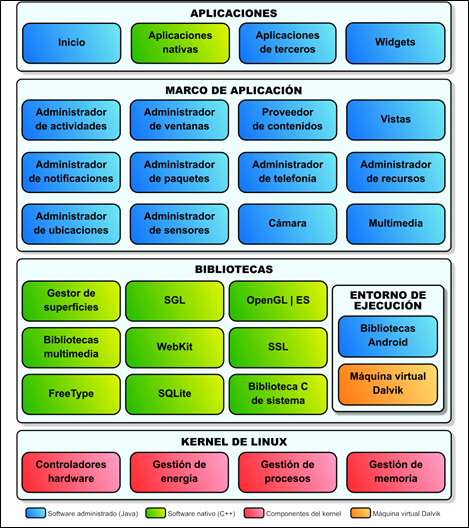
\includegraphics[scale=0.55]{C:/Users/usuario/Tesisworkspace/Tesis_Standalone/tesis/images/Android-architecture}
\par\end{centering}

\caption{Diagrama de la arquitectura en capas empleada por Android\label{fig:Android-architecture}}
\end{figure}


Las capas interactúan entre sí respetando el estilo arquitectónico
tradicional, donde cada una de las capas utiliza los servicios ofrecidos
por las anteriores, y ofrece a su vez sus propios servicios a las
capas de niveles superiores. 

Las diferentes capas de la arquitectura son descritas a continuación:
\begin{itemize}
\item Kernel Linux: Android utiliza el núcleo de Linux como una capa de
abstracción de hardware para los dispositivos móviles. Esta capa contiene
los drivers necesarios para que cualquier componente de hardware pueda
ser utilizado mediante las llamadas correspondientes, sólo debe considerarse
al momento de incluir un nuevo componente de hardware que los fabricantes
hayan desarrollado los drivers correspondientes. Además del soporte
de drivers, la capa es responsable de proporcionar otros servicios
como la seguridad, el manejo de la memoria, la gestión de procesos,
la pila de protocolos. 
\item Entorno de ejecución de Android: como se ha adelantado previamente,
cada aplicación corre en su propio proceso Linux con su propia instancia
de la máquina virtual Dalvik, la cual interpreta un lenguaje ligeramente
diferente al tradiciones de \ac{JVM} bajo el formato .dex. A partir
de la versión 5.0 de Android, Dalvik es reemplazada por \ac{ART}
la cual logra reducir el tiempo de ejecución del código Java hasta
un 33\%. También se incluye en el entorno un módulo de librerías nativas
con la mayoría de librerías disponibles en lenguaje Java. Estas bibliotecas,
si bien resultan diferentes a las ofrecidas por \ac{Java SE} y \ac{Java ME},
proveen prácticamente la misma funcionalidad. 
\item Bibliotecas: Incluye un conjunto de librerías en lenguaje C o C++
usadas en varios componentes de Android proporcionando la mayor parte
de las capacidades más características de Android, algunas de ellas
fueron expuestas en la figura anterior. En el caso de las bibliotecas
SQLite se provee acceso a la utilización y administración de bases
de datos \ac{SQL}. Estas librerías están compiladas en código nativo
del procesador y muchas de ellas utilizan proyectos de código abierto. 
\item Marco o entorno de Aplicaciones: Proporciona una plataforma de desarrollo
libre para aplicaciones con gran riqueza e innovaciones de herramientas
como sensores, localización, servicios, barra de notificaciones, entre
otros. y además permite que los desarrolladores tengan acceso a las
mismas \ac{API} utilizadas por las aplicaciones base del sistema.
El foco principal del diseño de esta capa ha sido simplificar la reutilización
de componentes, las aplicaciones pueden publicar sus capacidades y
otras pueden hacer uso de ellas (sujetas a restricciones de seguridad),
un mecanismo que permite a los usuarios reemplazar fácilmente componentes. 
\item Aplicaciones: Este nivel contiene todas las aplicaciones de usuario,
tanto las incluidas por defecto en Android así como como aquellas
que el usuario vaya añadiendo posteriormente ya sean de terceros o
de su propio desarrollo. Todas estas aplicaciones utilizan los servicios,
las \ac{API} y bibliotecas de los niveles inferiores. Se brindará
una descripción más detallada en la sección siguiente
\end{itemize}

\subsection{Aplicaciones Android \label{sec:Aplicaciones-Android}}

Además de las características técnicas, es importante resaltar que
la popularidad de Android ha crecido muy rápidamente desde su lanzamiento.
Esto se debe a la versatilidad que Android otorga a éstos dispositivos
a través de las aplicaciones, que permiten adaptarlos según las necesidades
de los usuarios. Además, el hecho de que Android sea de código abierto
da lugar a la creación de diferentes versiones del sistema operativo
que permiten personalizar cada aspecto del mismo. Android también
permite que las aplicaciones se adapten a las características del
dispositivo (pantalla, sensores, etc.), aprovechando las capacidades
de cada dispositivo particular. 

Respecto a las herramientas de desarrollo, Android ofrece un paquete
que combina el \ac{IDE} Eclipse con un conjunto de herramientas que
simplifican el desarrollo, permitiendo incluso, crear dispositivos
virtuales que emulan cualquier configuración de hardware soportada. 

Por otra parte, en el contexto de los servicios Web, Android provee
soporte para conexiones \ac{HTTP} , y por tanto, permite la utilización
de servicios Web \ac{REST} a través de ella. 

Un aspecto único del diseño de las aplicaciones en Android es que
éstas pueden reutilizar componentes de otras aplicaciones instaladas
en el dispositivo. Por ejemplo, si una aplicación desea tomar una
fotografía, es probable que ya exista una aplicación que cumpla esa
funcionalidad, entonces, la nueva aplicación puede utilizar la existente
sin necesidad de desarrollar una actividad propia para utilizar la
cámara, esta invocación se realiza de modo tal que sea transparente
para el usuario final.

El sistema Android provee cinco tipos de componentes básicos para
el desarrollo de aplicaciones. El componente \emph{Activity }representa
una pantalla simple y es el único que provee interfaz de usuario.
A través de estas actividades se logra el acceso a la información
almacenada en los componentes \emph{Content Provider }que son los
encargados de administrar la información compartida por las aplicaciones;
las aplicaciones pueden almacenar sus datos en el sistema de archivos,
en una base SQLite, en la Web, o en cualquier otro lugar de acceso.
A través del ‘content provider’, otras aplicaciones pueden consultar,
o incluso modificar estos datos. 

Las actividades también pueden iniciar servicios que se ejecutan en
segundo plano para realizar operaciones que requieran gran cantidad
de tiempo, o interactúen con procesos remotos, por ejemplo la reproducción
de música en segundo plano o la descarga de datos mientras el usuario
interactúa con una aplicación diferente. 

Respecto a los anuncios o mensajes de difusión masiva, el componente
\emph{Broadcast Receiver} funciona como puerta de enlace a otros componentes,
respondiendo mayormente a los anuncios originados por el sistema,
por ejemplo, cuando la pantalla se apaga, la batería es baja, o al
capturar una fotografía. 

El último componente denominado \emph{Intent} representa acciones
a realizar, específicamente, tienen por finalidad iniciar actividades,
servicios o \emph{Broadcast Receivers} realizando el binding en tiempo
de ejecución entre los componentes de las aplicaciones (tanto entre
componentes de una misma aplicación como de diferentes). Cada Intent
cuenta con una estructura de datos donde se realiza una descripción
abstracta de una operación a realizar, luego, la entrega de estos
objetos se realiza de diferente manera de acuerdo el tipo de componente
que se desee activar. 


\section{Componentes de software\label{sec:Componentes-de-software}}

En el marco del desarrollo de software para diferentes plataformas
y para móviles más específicamente, nos encontramos con la posibilidad
de reutilizar código previamente desarrollado, testeado y deployado
que cumpla con una determinada funcionalidad ahorrando tiempo y esfuerzo
al desarrollador. Estas piezas de códigos ya implementadas y disponibles
se conocen bajo el nombre de componentes de software e incluyen en
su definición paquetes de software, servicios o recursos web, o módulos
que encapsulan a un conjunto de funciones o datos relacionados; sin
embargo, cualquiera sea la pieza que represente, frecuentemente los
componentes son vistos y tratados como objetos o colección de objetos. 

La reutilización es uno de los objetivos principales al momento de
diseñar un nuevo componente de software de gran calidad para ser usados
en diferentes programas. Por lo tanto la implementación y diseño de
un componente conlleva un gran esfuerzo e incluye procesos complejos
como la documentación, testing robusto a través de entradas comprensibles
y la posibilidad de retornar mensajes de error y códigos, y el diseño
enfocado a la utilización en formas imprevistas. Si bien los componentes
actúan sin modificar su código, el comportamiento de los códigos fuentes
del componente puede cambiar basado en la extensibilidad de la aplicación. 

Todos los procesos de sistemas son estructurados bajo componentes
separados de modo tal que todos los datos y funciones de un componente
mantengan una misma relación semántica, principio que se mantiene
en el contenido de las clases. Por esta razón, se le atribuye a los
componentes las características de ser modulares y cohesivos. 

La comunicación entre componentes se realiza a través de interfaces.
Cuando un componente ofrece servicios al resto del sistema, el mismo
proporciona una interfaz que especifica los servicios que otros componentes
pueden utilizar y la manera en que pueden hacerlo. La interfaz puede
verse como una firma del componente ya que el cliente no necesita
conocer el procesamiento interno del componente para utilizarlo, condición
que respeta el principio de encapsulamiento. 

Por otro lado, cuando un componente necesita de otro para su funcionamiento,
el mismo establece las interfaces requeridas donde especifica los
servicios que necesita. 

De acuerdo al modelo \ac{UML} y lo reflejado en la figura \ref{fig:UML-component},
las interfaces proporcionadas son representadas con símbolos de lollipop
en el borde del componente y las interfaces requeridas por medio de
sockets abiertos en el borde externo. 

\begin{figure}
\begin{centering}
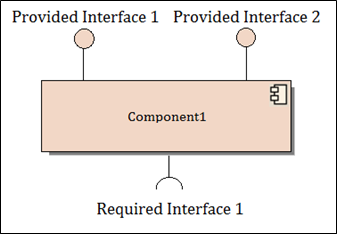
\includegraphics[scale=0.55]{C:/Users/usuario/Tesisworkspace/Tesis_Standalone/tesis/images/UML-component}
\par\end{centering}

\caption{Componente UML con interfaces proveídas y requeridas.\label{fig:UML-component}}
\end{figure}


Otra de las características fundamentales de los componentes es su
capacidad de ser sustituibles tanto en tiempo de diseño como en tiempo
de ejecución, pudiendo ser reemplazados por actualizaciones u otras
alternativas sin romper el sistema en el que los componentes funcionan.
El reemplazo es posible si el componente sucesor provee por lo menos
la misma funcionalidad que el componente a reemplazar y si requiere
a lo sumo las mismas funciones que el componente inicial. 


\section{Atributos de calidad \label{sec:Atributos-de-calidad}}

Al diseñar un sistema de software no sólo se espera cumplir con los
objetivos de negocio sino también alcanzar un determinado grado de
calidad de software capaz de satisfacer al grupo de usuarios y/o diseñadores,
muchos factores determinan las cualidades que deben proporcionarse
en la arquitectura de un sistema. Estas cualidades \cite{Ghahramani2004}
van más allá de la funcionalidad (capacidades), servicios y comportamientos
del sistema El diseño de la arquitectura de un sistema depende mayormente
de los atributos de calidad (también denominados propiedades no funcionales)
demandados por los stakeholders que de la funcionalidad en sí misma
que especifica el comportamiento que debería tener el producto, para
considerar un software de utilidad; largos tiempos de respuesta, caídas
del sistema, interfaces confusas, no son características deseables
en un sistema, por lo que toda decisión respecto al diseño de la arquitectura
debe conducir al cumplimiento de ciertos atributos de calidad al mismo
tiempo que cumple con la funcionalidad requerida. 


\subsection{Performance\label{subsec:Atributos-de-calidad-Performance}}

Se puede medir la calidad de un sistema a través de su desempeño evaluando
la efectividad del uso de los recursos disponibles en tiempo de ejecución.
Dependiendo el contexto, la eficiencia puede medirse a través de varios
parámetros, incluyendo tiempo de respuesta, ancho de banda y disponibilidad. 

El rendimiento de un sistema engloba, generalmente, el tiempo de los
eventos que se producen y que el sistema debe responder a ellos. Estos
eventos pueden ser muy variados tales como alarmas, mensajes, peticiones
a usuarios o simplemente tiempo de procesamiento, pero básicamente
se considera de todos ellos el tiempo que tarda el sistema para responder
ante el evento . La complejidad para el manejo de estos eventos radica
en su fuente, ya que pueden provenir desde una solicitud de usuario,
de otros sistemas o desde el interior del propio sistema. 

Sin importar el contexto de desarrollo del sistema, el patrón de los
eventos que llegan y el patrón de respuestas se pueden caracterizar,
y esta caracterización hace posible la construcción de escenarios
generales de rendimiento empleados en diferentes benchmarks, por ejemplo
el tiempo de respuesta puede significar el tiempo máximo y mínimo
de procesamiento para cierto elemento del sistema o la cantidad máxima
de eventos que un determinado servicio puede atender por unidad de
tiempo. 

La respuesta del sistema a un estímulo puede ser caracterizado por
la latencia (el tiempo entre la llegada del estímulo y la respuesta
del sistema a la misma), los plazos de procesamiento, la fluctuación
de la respuesta (la variación de latencia), el número de eventos no
procesados debido a que el sistema era demasiado ocupado para responder,
y los datos que se perdió debido a que el sistema era demasiado ocupado. 


\subsection{Precisión\label{subsec:Atributos-de-calidad-Precisi=0000F3n}}

Cabe destacar que no existe una definición estándar sobre el significado
de precisión en un sistema, ya que se trata de una medida que evalúa
qué tan exacta es la respuesta de un componente, y cada componente
está fuertemente ligado al dominio en el que se presenta, por ejemplo,
en un problema de detección de rostros, la precisión puede significar
la cantidad de rostros correctamente detectados sobre los rostros
totales presentes, y en un problema de clasificación puede significar
la correctitud en la predicción de la clase para un cierto atributo.

En términos generales, se toma la precisión como el grado de cercanía
(o dispersión) de las mediciones respecto al verdadero valor, es el
grado en que si las mediciones se repitieran bajo las mismas condiciones
los resultados serían los mismos. A menudo, la medida de precisión
es confundida con el término exactitud que indica la distancia del
valor medido respecto al valor verdadero. Por ejemplo, si un experimento
contiene un error sistemático, el aumento del tamaño de la muestra
en general aumenta la precisión, pero no mejora la exactitud. El resultado
sería una cadena consistente (aunque incorrecto) de los resultados
del experimento defectuoso. La eliminación del error sistemático mejora
la exactitud, pero no cambia la precisión. 


\section{Aprendizaje de máquina \label{sec:Aprendizaje-de-maquina}}

El aprendizaje a partir de datos es la base para comprender el proceso
de aprendizaje de máquina ya que los datos son la única herramienta
de la que se dispone y conoce a ciencia cierta sobre las características
de un dominio cualquiera. La representación de los datos reales puede
alcanzar el tamaño de terabytes por lo que dificulta hacer una analogía
respecto al aprendizaje humano basado en la experiencia. 

El hombre basa su conocimiento en tres partes: \emph{i}) recuerdo,
el hombre reconoce cuando ha sido la última vez que se estuvo en una
determinada situación (dataset), \emph{ii}) adaptación, reconoce la
última vez que se probó una acción (salida producida) y \emph{iii})
generalización, si ha funcionado o no (si fue correcta o no). 

El término generalización refiere a la similitud entre diferentes
situaciones de manera tal que las opciones que han sido aplicadas
en casos previos pueden ser usadas en nuevos casos. Estas fueron las
bases del primer Aprendizaje Artificial y es conocido como procesamiento
de símbolos ya que las computadoras manipulan símbolos que reflejan
el ambiente. En contraste, los métodos de aprendizaje de máquinas
son llamados sub-simbólicos ya que no se utilizan símbolos. 

El aprendizaje de máquina, entonces, es un proceso para que las computadoras
modifiquen o adapten sus acciones (predictivas o de control de robot)
para que sus resultados sean más precisos, precisión que refleja la
proximidad respecto a las acciones correctas. El aprendizaje de máquina
reúne ideas de neurociencia y biología, estadística, matemática y
física, para generar técnicas y hacer que la computadora aprenda.
Otro concepto importante en este ámbito es la minería de datos, el
proceso de extraer información útil de un conjunto de datos masivos
llamado comúnmente dataset por medio de algoritmos de alto grado de
eficiencia y enfatizados nuevamente en la ciencia computacional. 

Quizás, el punto de inflexión en este campo de estudio es la complejidad
computacional de la aplicación de técnicas de aprendizaje de máquina
sobre un gran volumen de datos, de manera que los algoritmos de complejidad
polinomial muy grande pueden resultar un problema. Generalmente la
complejidad se divide en dos partes: la complejidad del entrenamiento
y la complejidad de aplicar el algoritmo entrenado. El proceso de
entrenamiento usualmente, se realiza escasas veces, incluso tan sólo
una, y el tiempo que requiere no resulta tan crítico, por lo que se
enfatiza sobre la segunda parte donde se pretende que la decisión
sea lo más rápida posible con un bajo costo computacional. 

Si se define en forma imprecisa el concepto de aprendizaje como la
mejora de tareas a través de la práctica surgen algunos cuestionamientos
asociados, de qué forma la computadora puede saber si está aprendiendo
mejor o de qué forma podría mejorar ese aprendizaje. De aquí, toman
lugar diferentes tipos de aprendizaje de máquina, por ejemplo se le
puede indicar a un algoritmo la respuesta correcta para un problema,
así, la próxima vez que se aplique su desempeño será mejor. También,
podría indicarse un conjunto de respuestas correctas para que la máquina
\emph{adivine} la forma de obtener estas respuestas para otros problemas
(generalización). Alternativamente, se puede indicar si la respuesta
obtenida es correcta o no sin señalar la respuesta real ya que la
máquina debería ser capaz de encontrarla; una variante podría ser
asignarle un puntaje a la respuesta obtenida por el algoritmo acordando
cuán correcta resulta ser y no sólo indicarlo mediante los valores
verdadero o falso. 

Estas diferentes respuestas proveen una forma fácil de clasificar
los diferentes métodos de aprendizaje, los cuales serán detallados
en las secciones siguientes en base a la naturaleza de la entrada
y la naturaleza de la salida; sin embargo todos los métodos comparten
el mismo objetivo de generalización: el algoritmo debe producir salidas
sensibles para datos de entrada que no fueron encontrados durante
el aprendizaje teniendo en cuenta también que el algoritmo puede lidiar
con ruido en los datos, una pequeña imprecisión en los valores que
es inherente a la medición de cualquier proceso real. 


\subsection{Clasificación por la naturaleza de la entrada}

El modo de aprendizaje que un algoritmo particular puede realizar
queda determinado por la naturaleza de los datos de entrada, es decir,
puede variar en base a la información contenida en los datos de entrenamiento
(\emph{training set}). 

El aprendizaje supervisado utiliza un conjunto de datos basado en
dos pares de objetos: los datos de entrada o conjunto de ejemplos
del dominio y las respuestas correctas (\emph{targets}) para una determinada
característica; a través de las respuestas correctas provistas y basado
en el conjunto de datos el algoritmo de aprendizaje generaliza el
comportamiento para responder a todas las posibles entradas. Este
modo de aprendizaje, entonces, es un proceso que se realiza mediante
un entrenamiento controlado por un agente externo que determina la
respuesta que debería generar el algoritmo a partir de una entrada
determinada. 

Contrariamente, el aprendizaje por refuerzo se basa en la idea de
no disponer de ejemplos completos del comportamiento deseado por el
algoritmo, es decir, no indicar durante el entrenamiento exactamente
la salida que se desea proporcione el clasificador ante una determinada
entrada, sólo se le indica si la salida obtenida se ajusta a la deseada
y en función a ello se re configuran los pasos. 

Por último, en el aprendizaje \cite{Ghahramani2004} no supervisado,
la máquina simplemente recibe los datos de entrada sin etiquetas o
respuestas correctas como en el método supervisado ni valores de recompensa
desde el ambiente, dando lugar a una percepción misteriosa sobre la
forma que se espera que el método aprenda sin recibir ningún tipo
de devolución. Sin embargo, es posible desarrollar un framework formal
para llevar a cabo aprendizaje no supervisado basado en la noción
de que el objetivo es construir una representación de la entrada que
puede ser usada para tomar decisiones, predecir futuras entradas,
comunicar eficientemente entradas para otras máquinas, entre otras
posibilidades. El aprendizaje no supervisado puede entenderse como
la búsqueda de patrones en los datos independientemente del ruido
presente en los mismos. 

Nótese que los valores de entrada y etiqueta describen vectores ya
que cada ejemplo (\emph{instance}) del conjunto de entrenamiento posee
varias características (\emph{features}); si se tuvieran todos los
posibles ejemplos de un problema, no habría necesidad alguna de aprendizaje.


\subsection{Clasificación por la naturaleza de la salida}

La teoría de aprendizaje de maquinas abarca varios factores considerando
las características de lo que se busca en los diferentes métodos.
Así, existen cinco tipos de métodos, para la búsqueda de diferentes
objetivos:
\begin{description}
\item [{Clasificación}] Consiste en asignar a cada ejemplo una etiqueta
o clase a la que pertenece basado en el entrenamiento de ejemplares
de cada clase. Los datos de entrenamiento son instancias que pertenecen
a una única clase y el conjunto de clases cubre todas las salidas
posibles, por eso se considera al proceso de clasificación como un
proceso discreto. El algoritmo de clasificación tiene como objetivo
encontrar umbrales de decisión que sirvan para identificar las diferentes
clases.
\item [{Clustering}] El proceso de clustering es la tarea de agrupar un
conjunto de objetos de modo tal que los objetos pertenecientes a un
mismo grupo (\emph{cluster}) comparten algún tipo de similitud entre
ellos, de igual sentido que se diferencian con los objetos de otro
grupo. A diferencia del proceso de clasificación, los grupos o clases
no son conocidos fehacientemente antes del entrenamiento, un claro
método de aprendizaje no supervisado. 
\item [{Estimación~de~densidad}] La función de densidad de probabilidad
\cite{Silverman1986} es un concepto fundamental de la estadística
y caracteriza el comportamiento probable de una población en tanto
especifica la posibilidad relativa de que una variable aleatoria continua
X tome un valor cercano a x.
\item [{Reducción~de~dimesionalidad}] Se basa en simplificar los datos
de entrada mapeándolos en un espacio dimensional más simple.
\item [{Regresión}] El proceso de regresión predice valores numéricos de
atributos a partir de funciones matemáticas polinomiales que describan
o se ajusten lo más posible a todos los puntos del dominio, es decir,
todos los valores del conjunto de entrenamiento correspondientes al
atributo que se quiere predecir. Generalmente, se considera un problema
de aproximación de función o interpolación al encontrar un valor numérico
entre los valores conocidos. Por lo tanto, el eje primordial del proceso
de regresión es encontrar la función que mejor represente al conjunto
de puntos, ya que funciones con distintos grados de polinomios causan
diferentes efectos. La figura \ref{fig:regression-problems} refleja
la situación expresada anteriormente, donde se muestra el conjunto
de valores del dominio y tres curvas alternativas de representación.
El gráfico inferior izquierdo combina, además, una función cúbica
y línea recta. 
\end{description}
\begin{figure}
\begin{centering}
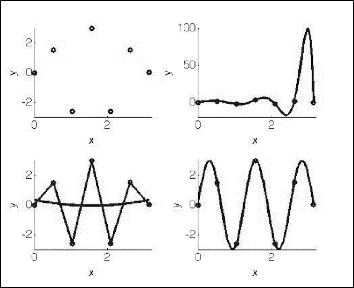
\includegraphics[scale=0.55]{C:/Users/usuario/Tesisworkspace/Tesis_Standalone/tesis/images/regression-problems}
\par\end{centering}

\caption{Comparación de distintas funciones polinomiales de regresión. \label{fig:regression-problems}}
\end{figure}


La forma más correcta de saber cuál solución presentada es la mejor,
se evalúa el grado de generalización que permite cada una; se toma
algún punto incluido entre los puntos ya representados y se utiliza
la curva para predecir el valor, luego se compara entre los valores
para saber cual resultó más próximo. En este caso, el gráfico inferior
derecho. 

~

Cabe destacar que en el presente trabajo, se analizan técnicas de
regresión, ya sea aquellas que intrínsecamente representan funciones
polinomiales como aquellas que se adaptaron desde los métodos de clustering
para la obtención de valores densos.


\subsection{Funciones contempladas\label{subsec:Funciones-contempladas}}

El foco principal del trabajo desarrollado ha sido guiado por la búsqueda
de predicción de valores numéricos sobre componentes de ejecución,
como el uso de CPU, consumo de red, precisión y desempeño de las respuestas,
entre otros. Estos indicadores son valores continuos, motivo por el
cual se utilizaron modelos de regresión, los mismos se describirán
en las subsecciones siguientes. 


\subsubsection{Regresión Lineal\label{sub:Regresi=0000F3n-Lineal}}

La regresión es la predicción de un valor desconocido a través del
cálculo de una función matemática a partir de los valores conocidos.
Si se considera esta función como una línea recta, la salida será
la suma de cada valor conocido multiplicado por una constante la cual
define la línea recta (plano en 3D o hiperplano en dimensiones mayores)
que circundan los puntos como puede observarse en la figura \ref{fig:regression-lineal}. 

\begin{figure}
\begin{centering}
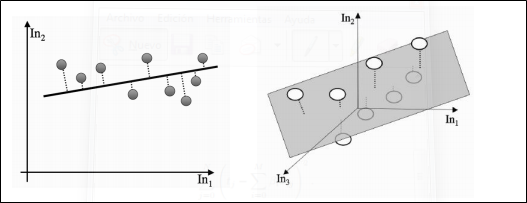
\includegraphics[scale=0.55]{C:/Users/usuario/Tesisworkspace/Tesis_Standalone/tesis/images/regression-lineal}
\par\end{centering}

\caption{Algoritmo Linear regression en dos y tres dimensiones.. \label{fig:regression-lineal}}
\end{figure}


Para encontrar la recta que mejor se adapte a los datos se intenta
minimizar la distancia entre cada punto y dicha línea, esta distancia
se mide a través de una línea auxiliar que atraviese el punto y tope
con la función, por ejemplo mediante el Teorema de Pitágoras. Luego,
se intentará minimizar la función de error que mide la suma de cada
distancia, si se ignora las raíces y sólo se minimiza la suma de los
cuadrados de los errores, se obtiene la minimización más común llamada
optimización de mínimos cuadrados. 

La minimización de esta función da lugar a la implementación de diversas
alternativas de la función lineal. En el presente trabajo se desarrollan
dos variantes, la función denominada \emph{ridge-regression }y la
función \emph{gradiente estocástico descendiente}. La primera aplica
una penalización (\emph{ridge}) a cada constante. La segunda, aplica
un diferencial sobre la función obteniendo el gradiente el cual por
definición, es la dirección en la que incrementa o disminuye en mayor
medida. Ya que el propósito del aprendizaje es minimizar el error
de predicción, se debe seguir la función en dirección del gradiente
negativo en la cual la función disminuye. 


\subsubsection{Red neuronal}

Se presenta un modelo matemático sobre el comportamiento de una neurona,
el modelo neuronal McCulloch - Pitts denominado así debido a sus creadores
Warren McCulloch y Walter Pitts, ambos produjeron un ejemplo perfecto
al modelar una célula nerviosa como \emph{i}) un conjunto de entradas
valoradas (w\textsubscript{i}) que corresponde a las sinapsis, \emph{ii})
un sumador que une las señales entrantes (equivalente a la membrana
de la célula que recolecta la carga eléctrica) y \emph{iii}) una función
de activación (inicialmente una función umbral) que decide sobre la
activación de la célula en base a las entradas actuales. 

\begin{figure}
\begin{centering}
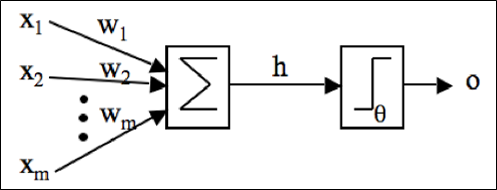
\includegraphics[scale=0.55]{C:/Users/usuario/Tesisworkspace/Tesis_Standalone/tesis/images/McCulloch-Pitts}
\par\end{centering}

\caption{Modelo matemático neuronal McCulloch - Pitts. \label{fig:McCulloch-Pitts}}
\end{figure}


Como puede observarse en la figura \ref{fig:McCulloch-Pitts}, el
modelo McCulloch - Pitts es un dispositivo límite binario, las entradas
son multiplicadas por los pesos o fuerzas sinápticas y luego se suman
sus valores, si la suma es mayor a un determinado umbral (produce
salida 1) la célula se activa, de lo contrario (produce salida 0)
se mantiene desactivada. Teniendo en cuenta que una red neuronal puede
llevar a cabo cualquier cálculo que realiza una computadora normal,
los pesos o valores de la fuerza sináptica deben ser elegidos correctamente,
considerando en consecuencia, un método capaz de configurar dichos
pesos. Observando la neurona McCulloch y Pitts, se puede notar fácilmente
que las entradas son independientes al cerebro, por lo que sólo cambia
el valor de los pesos y el umbral. Considerando que el aprendizaje
sucede entre las neuronas y éstas están conectadas mutuamente, se
debe tener en cuenta la manera en que en cambian los pesos y los umbrales
de las neuronas para que la red pueda obtener la respuesta correcta
más frecuentemente.

Teniendo en cuenta que una red neuronal puede llevar a cabo cualquier
cálculo que realiza una computadora normal, los pesos o valores de
la fuerza sináptica deben ser elegidos correctamente, considerando
en consecuencia, un método capaz de configurar dichos pesos.

Observando la neurona McCulloch y Pitts, se puede notar fácilmente
que las entradas son independientes al cerebro, por lo que sólo cambia
el valor de los pesos y el umbral. Considerando que el aprendizaje
sucede entre las neuronas y éstas están conectadas mutuamente, se
debe tener en cuenta la manera en que en cambian los pesos y los umbrales
de las neuronas para que la red pueda obtener la respuesta correcta
más frecuentemente. 


\subsubsection*{Red Neuronal Perceptron }

El perceptrón es una colección de neuronas McCulloch y Pitts con un
conjunto de entradas y pesos que unen las neuronas con dichas entradas. 

\begin{figure}
\begin{centering}
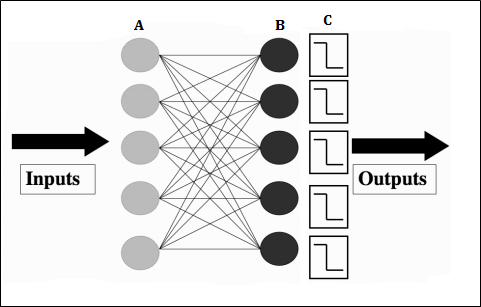
\includegraphics[scale=0.55]{C:/Users/usuario/Tesisworkspace/Tesis_Standalone/tesis/images/perceptron-neural-network}
\par\end{centering}

\caption{Red neuronal perceptron\label{fig:perceptron-neural-network}}
\end{figure}


Como puede observarse en el gráfico de la figura \ref{fig:perceptron-neural-network},
las neuronas del Perceptrón son completamente independientes entre
sí, el estado de una neurona no infiere sobre las demás, sólo comparten
las entradas. Un punto a destacar es que el número de entradas y de
neuronas no necesariamente debe corresponderse, en general hay \emph{m}
entradas y \emph{n} neuronas. 

El mayor inconveniente es conocer con certeza los valores que deben
tener los pesos para que las salidas sean las correctas, esta es la
finalidad de la red neuronal, aprender si determinada neurona debe
o no activarse de forma correcta. 

Un proceso de análisis sobre los pesos podría arrojar que los pesos
toman valores muy grandes en la activación de una neurona (cuando
no debería hacerlo) o en caso contrario, valores muy pequeños, por
lo que se podría computar una función de error como la diferencia
entre la salida que produjo la neurona y la salida de la red. En el
caso particular de entradas en cero, se modifica el valor de umbral
añadiendo a la red Perceptron un parámetro extra denominado bias,
los pesos de esta entrada son usualmente asignados al índice cero. 


\subsubsection*{Red neuronal Perceptrón multicapa }

La esencia del aprendizaje de la red neuronal perceptrón está centrada
en los valores de pesos, una buena práctica entonces, sería la incorporación
de nuevos pesos. Como alternativa para ello podrían agregarse conecciones
hacia atrás para conectar las neuronas de salida con las entradas
nuevamente, o podrían agregarse nuevas neuronas creando redes mucho
más complejas, como el caso reflejado en la figura \ref{fig:perceptron-neural-network-multilayer}
donde se representa un modelo perceptrón de tres capas con cinco entradas,
tres salidas y tres neuronas en la capa oculta.

\begin{figure}
\begin{centering}
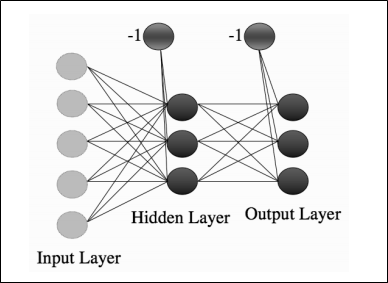
\includegraphics[scale=0.55]{C:/Users/usuario/Tesisworkspace/Tesis_Standalone/tesis/images/Perceptron-multilayer}
\par\end{centering}

\caption{Red perceptrón multicapa\label{fig:perceptron-neural-network-multilayer}}
\end{figure}


La nueva red, ahora, debe ser entrenada para que los pesos nuevos
se adapten y generen las respuestas correctas (\emph{targets}). Estas
respuestas son conocidas y se puede computar la diferencia entre estas
y las salidas pero se desconoce si el peso incorrecto pertenece a
la primera capa o a la segunda y cuáles activaciones de las neuronas
de la capa intermedia son correctas, razón por la cual esta capa se
denomina capa oculta ya que es imposible examinar y corregir sus valores
de forma inmediata. 

El entrenamiento de \ac{MLP} consiste en dos partes, primero se obtienen
las salidas con las entradas brindadas y los pesos actuales (\emph{forwards}),
y luego se actualizan los pesos considerando el error como la diferencia
entre el valor obtenido y el real (propagación hacia atrás del error
- \emph{backwards}). 

Por lo tanto, con la función de error y de activación, puede calcularse
el diferencial para modificar los pesos en dirección del gradiente
negativo, mejorando así la función de error. El objetivo es obtener
los gradientes de esos errores y usarlos para decidir cuánto deben
actualizarse dichos pesos en la red sobre la capa de salida y, luego
de actualizarla, se opera hacia atrás (\emph{backwards}) a través
de la red hasta llegar a la entrada nuevamente. Sólo existen dos problemas,
para las neuronas de salida se desconocen las entradas que le corresponden
y para las neuronas escondidas, se desconocen las salidas esperadas
(\emph{targets}) y en caso de existir más capas incluso podrían no
conocerse las entradas. Para solucionar estas cuestiones se aplica
la regla de la cadena la cual afirma que para conocer la forma en
que varía el error en base a la variación de los pesos, se debe analizar
la variación del error en función de las entradas de los pesos y multiplicarlo
por el valor de la variación de los pesos según la variación de entradas. 

Esta forma de resolución es muy útil ya que permite conocer todas
las derivadas que se necesitan. Puede escribirse la función de activación
de los nodos de salida en términos de los nodos ocultos y de los pesos
de salida para luego enviarlo hacia las capas ocultas de la red (hacia
atrás) para decidir cuáles eran los salidas esperadas para esas neuronas.


\subsubsection{K-means clusterer}

El algoritmo K - means aplica clustering sobre los datos de entrenamiento
y recibe un parámetro \emph{K} para dividir estos datos en \emph{K}
categorías. El algoritmo intenta localizar k centros en el espacio
de entrada de modo tal que estos centros estén, como su nombre lo
indica, en el centro de una categoría (\emph{cluster}). La dificultad
se presenta ya que al desconocer la categorización de estos grupos,
resulta aún más difícil determinar la localización de cada centro. 

Los algoritmos de aprendizaje generalmente se basan en minimizar alguna
clase de error, en consecuencia la primera acción que se realiza es
definir un criterio que lo describa teniendo en cuenta: \emph{i})
una medida de la distancia entre puntos, definir una medida para cuantificar
estas distancias, por lo general se usa la distancia euclídea y \emph{ii})
determinar el punto central de un conjunto de puntos (\emph{mean average})
considerando el espacio euclídeo ya que en espacios curvos es otra
la interpretación. Teniendo en cuenta estos conceptos, el algoritmo
K - means calcula el punto medio (centro) de cada cluster (µ\textsubscript{c}(i)).
lo que resulta equivalente a minimizar la distancia euclídea de cada
punto del cluster al centro del mismo. 

El objetivo de determinar estos centros, en principio, a causa de
incertidumbre total se posicionan los centros de forma aleatoria en
el espacio de entrada. Una vez distinguidos los clusters, se determinar
los puntos que pertenecen al mismo a través del cálculo de la distancia
entre el punto y todos los centros localizados, asignándose entonces,
al cluster cuyo centro sea el más cercano. Finalmente, para cada centro
se actualiza su ubicación utilizando la media antes definida. Estos
pasos se realizan de forma incremental hasta que los centros dejar
de modificar su ubicación. 

Ya que este algoritmo sin duda es un método de clasificación y no
de regresión, se considera importante resaltar la adaptación del mismo
para utilizarlo con este fin. Así, una vez realizada la clasificación
del punto que se quiere predecir, se realizará la predicción calculando
el promedio de los valores del atributo a predecir de los otros puntos
que están en el cluster. 


\subsubsection{Maquina de vector de soporte}

Al tratar con problemas de clasificación existen varios clasificadores
lineales que ofrecen respuestas correctas pero diferentes, como se
expone en la figura \ref{fig:lineals-classifiers}. Si bien las soluciones
laterales son acertadas, las líneas divisorias son muy próximas a
algunos puntos del conjunto de datos de entrenamiento dando paso a
una posible imprecisión futura en la predicción, situación que no
se observa en el ejemplo central de la figura. 

\begin{figure}
\begin{centering}
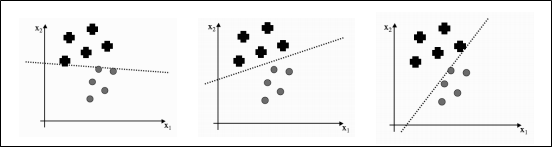
\includegraphics[scale=0.55]{C:/Users/usuario/Tesisworkspace/Tesis_Standalone/tesis/images/lineals-classifiers}
\par\end{centering}

\caption{Comparación de tres clasificadores lineales distintos.\label{fig:lineals-classifiers}}
\end{figure}


Analíticamente, se toma la distancia existente entre la línea y el
primer punto interceptado (en dirección perpendicular), si se ubica
una ‘zona desierta’ alrededor de la línea, ningún punto ubicado en
dicha zona puede ser clasificado ya que se encuentra demasiado cerca
de la línea. Esta región conforma un cilindro simétrico alrededor
de la función en 3D y un hiper - cilindro en dimensiones mayores.
El radio máximo que puede tener esta región es llamado margen, señalado
como M y los puntos de cada clase más cercanos a la línea de clasificación
se denominan vectores de soporte. Si se considera el mejor clasificador
como aquel que atraviesa la zona desierta, se debe tener en cuenta
que el margen debe ser lo más grande posible y que si los vectores
de soporte son los puntos más importantes de los datos, luego del
entrenamiento pueden descartarse los puntos que no pertenecen al vector
y utilizarlos para clasificar, lo cual conlleva una gran eficiencia
en el almacenamiento de datos. El algoritmo puede encontrar varios
hiperplanos de separación posibles y detectar aquel que sea más óptimo.
En la figura \ref{fig:SVM-metology} se reflejan estas dos situaciones
y se expone, en el gráfico derecho las notaciones matemáticas formales
del algoritmo. 

\begin{figure}
\begin{centering}
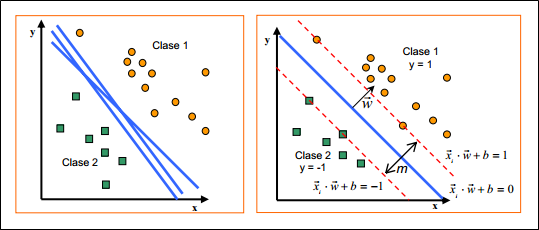
\includegraphics[scale=0.55]{C:/Users/usuario/Tesisworkspace/Tesis_Standalone/tesis/images/SVM-metology}
\par\end{centering}

\caption{Metodología de operación del algoritmo SVM\label{fig:SVM-metology}}
\end{figure}


A través de la función \emph{g(x) = w\textsuperscript{t}x + b} se
definen los dos hiperplanos (clasificador). Para obtener el punto
más cercano desde la línea de clasificación considerando la clase
2 (ver figura \ref{fig:SVM-metology}) se recorre en dirección perpendicular
partiendo del límite de la clase 1 hasta llegar al límite de la clase
2, el primer punto interceptado se denomina x. Para obtener un clasificador
de buena calidad, se pueden definir un conjunto de restricciones que
indiquen la manera en que el clasificador podría obtener la respuesta
correcta. Por ejemplo, si en lugar de tomar las dos clases como \emph{g(x)
= 1} y \emph{g(x) = 0}, se podrían igualar a los valores 1 y -1 y
así obtener una respuesta correcta diferente. Estos tipos de problemas
pueden ser resueltos de forma directa y eficiente (por ejemplo, en
tiempo polinomial), gracias a que existen algoritmos de programación
cuadrática que brindan soluciones efectivas.

Todas las consideraciones expuestas hasta el momento se realizaron
tras la asunción de que los datos podían ser divididos con funciones
lineales, pero no siempre es posible, en este caso la solución es
introducir variables. Estas variables indican que, al comparar clasificadores,
si uno clasifica un punto en un lado incorrecto y el otro lo ubica
mucho más lejos (también en un lado incorrecto) el primero es mejor
que el segundo, el error no fue tan extremo como en el segundo y esta
información debe ser incluida en los criterios de minimización modificando
las restricciones, incluyendo un parámetro \emph{C}. \emph{C} es el
parámetro que indica el trade off que existe entre ambos parámetros:
cuanto más pequeño sea el valor de C más importancia toma el margen
sobre algunos errores, cuanto más grande se vuelve C ocurre lo contrario.
Esto transforma el problema en un clasificador de margen suave ya
que se permiten algunos errores. La forma de evitarlos es modificando
las características para que los datos sean linealmente separables,
los datos no pueden inventarse de modo que las características deben
ser derivadas a partir de las existentes. Para ello se describe una
nueva función llamada kernel denominada \emph{φ(x)} que se aplica
sobre las diferentes variables de entrada, su función principal es
transformar los datos para obtener un espacio de dimensión mayor.
Como función kernel puede utilizarse cualquier función simétrica que
está definida positivamente (positividad de la integral de funciones
arbitrarias). Incluso, la conjunción de dos funciones kernel significa
una nueva función kernel. Elegir la función kernel más conveniente
es un problema complejo. A pesar que existen algunas teorías, el proceso
más común es la experimentación con distintos valores para determinar
la función más adecuada utilizando el conjunto de validación. El algoritmo
que aplica vectores de soporte se rige bajo todos los conceptos expresados
a lo largo del apartado para realizar clasificación, pero también
aplica para realizar regresión sobre los datos, variante que fue utilizada
en el presente trabajo. La figura \ref{fig:SVM-regression} muestra
un ejemplo de la aplicación del algoritmo SVM para regresión. 

\begin{figure}
\begin{centering}
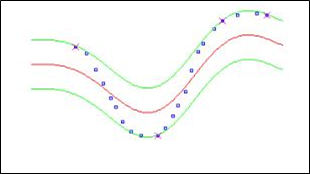
\includegraphics[scale=0.55]{C:/Users/usuario/Tesisworkspace/Tesis_Standalone/tesis/images/SVM-regression}
\par\end{centering}

\caption{Algoritmo SVM para regresión con función kernel de base radial.\label{fig:SVM-regression}}
\end{figure}



\subsection{Evaluación de modelos}

La evaluación del rendimiento de un modelo es una de las fases principales
en el proceso de ciencia de datos. Indica el nivel de acierto de las
predicciones del conjunto de datos mediante un modelo entrenado. Existen
dos formas para evaluar: evaluar el modelo y validar el modelo de
forma cruzada. Estos métodos permiten conocer el rendimiento del modelo
como un número de métricas que se usan habitualmente en estadísticas
y aprendizaje automático. La evaluación y la validación cruzada son
métodos estándares para medir el rendimiento de un modelo. Ambos generan
métricas de evaluación que sirven para inspeccionar y comparar con
las de otros modelos. 

La evaluación se basa en los valores predictivos junto con las etiquetas
o valores verdaderos. De forma alternativa, es posible usar la validación
cruzada para realizar automáticamente varias operaciones de entrenamiento,
puntuación y evaluación (10 subconjuntos) en distintos subconjuntos
de los datos de entrada. Los datos de entrada se dividen en 10 partes,
donde una se reserva para las pruebas y las otras 9 para el entrenamiento.
Este proceso se repite 10 veces y se calcula el promedio de las métricas
de evaluación. Esto ayuda a determinar el nivel al que un modelo se
podría generalizar para nuevos conjuntos de datos. 

El presente trabajo implementa las siguientes métricas de evaluación
para los modelos de regresión: 
\begin{itemize}
\item CC (Coeficiente de correlación de Pearson)
\item MAE (Mean Absolute Error) 
\end{itemize}
\[ \frac{1}{N}\sum_{i=1}^{N}{f_i-y_i}
\]
\begin{itemize}
\item RMSE (Root Mean Absolute Error)
\end{itemize}
\[ \sqrt{\frac{1}{N}\sum_{i=1}^{N}{f_i-y_i}^2}
\]
\begin{itemize}
\item RAE (Relative Absolute Error)
\end{itemize}
\[ \frac{\sum_{i=1}^{N}{|f_i-y_i}|}{\sum_{i=1}^{N}{|\overline{f_i}-y_i}|}
\]
\begin{itemize}
\item RRSE (Root Relative Squared Error)
\end{itemize}
\[ \sqrt{\frac{\sum_{i=1}^{N}{(f_i-y_i)^2}}{\sum_{i=1}^{N}{(\overline{f_i}-y_i)^2}}}
\]
\begin{itemize}
\item COMB
\end{itemize}
\[ (1-CC)+RRSE+RAE
\]
\begin{itemize}
\item SIMPLE ERROR
\end{itemize}
\[ \sum_{i=1}^{N}{(f_i-y_i)^2}
\]

El término \emph{error }representa la diferencia entre el valor predicho
y el valor verdadero. Normalmente, se calcula el valor absoluto o
el cuadrado de esta diferencia para capturar la magnitud total de
errores en todas las instancias, dado que la diferencia entre el valor
verdadero y el predicho puede ser negativa en algunos casos. Las métricas
de error miden el rendimiento de predicción de un modelo de regresión
en cuanto a la desviación media de sus predicciones a partir de los
valores reales. Los valores de error más bajos implican que el modelo
es más preciso a la hora de realizar predicciones. Una métrica de
error general de 0 significa que el modelo se ajusta a los datos perfectamente.


\subsection{Ajuste del modelo: Overfitting y Underfitting\label{sub:Ajuste-del-modelo:}}

Cuando un clasificador es entrenado se genera un modelo de predicción
cuya calidad es incierta hasta su aplicación. En algunas ocasiones,
la calidad del modelo es pobre generando respuestas imprecisas, de
modo tal que se le deben aplicar acciones correctivas comprendiendo
cómo se comporta y ajusta el modelo. 

Los modelos pueden presentar dos efectos indeseables . El efecto de
\emph{overfitting }describe una función que se ajusta estrechamente
a los datos de entrenamiento, el modelo aprendió los detalles y el
ruido en los datos impactando negativamente en el desempeño del modelo,
ha sido incapaz de generalizar. Este efecto es causado porque el ruido
o las fluctuaciones aleatorias en los datos de entrada fueron usados
para el aprendizaje. Los problemas de overfitting son más probables
en modelos no parametrizados y no lineales, los cuales tienen mayor
flexibilidad al aprender funciones. Por lo tanto, muchos algoritmos
de aprendizaje de máquina no parametrizados incluyen parámetros o
técnicas para limitar y restringir los detalles que el modelo aprende.
Por ejemplo, los árboles de decisión son algoritmos de aprendizaje
no parametrizados muy flexibles y pueden estar sujetos al efecto de
overfitting, en cuyo caso se procede a podar el árbol una vez que
el aprendizaje sea suficiente, eliminando así algunos detalles innecesarios.
Para solucionar este efecto se debe modificar el grado del polinomio
de la función utilizada por el modelo. 

Por otro lado, los modelos pueden presentar efectos de \emph{underfitting},
funciones que no interpretan o definen los datos de entrenamiento,
por lo que son incapaces de generalizar correctamente nuevos datos,
este efecto es causado porque la función o modelo elegido no es el
indicado para representar el comportamiento de los datos, el efecto
underfitting se caracteriza por sobre generalizar los datos. La incorporación
de nuevos datos al conjunto de entrenamiento podría solucionar o apaciguar
este efecto. 

El modelo deseado, sin dudas, sería aquel que se encuentre en un punto
de equilibrio entre modelos con underfitting y overfitting, aunque
esta eficiencia es muy difícil de alcanzar en la práctica. La figura
\ref{fig:under-overfitting} refleja el contraste entre los tres posibles
estados de un modelo. 

\begin{figure}
\begin{centering}
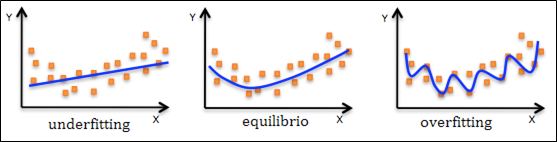
\includegraphics[scale=0.55]{C:/Users/usuario/Tesisworkspace/Tesis_Standalone/tesis/images/under-overfitting}
\par\end{centering}

\caption{Contraste entre distintos efectos del modelo sobre los datos de entrenamiento.\label{fig:under-overfitting}}
\end{figure}


El análisis de ambos efectos, se realiza gráficamente describiendo
la performance del algoritmo y la forma en que va aprendiendo a través
del tiempo. Al graficar la habilidad basada en los datos de entrenamiento
y en los datos de validación (testing), puede notarse que el error
basado en en el último gráfico de la figura \ref{fig:under-overfitting}
comienza a disminuir por efectos de overfitting ya que comienza a
aprender datos irrelevantes y ruidos del conjunto. En cuanto al gráfico
central (modelo esperado), se puede notar que el error aumenta mientras
el modelo aprender a generalizar. 

  
